\section{Quantum communication systems with PACSs}
    The effect of the use of PACS in an OOK communication system was extensively discussed in
    \cite{PACSDisc}. In this section the most important result will be reported and a BPSK
    system will be tested.

    \subsection{Quantum OOK}
    The use of PACS in an OOK system can significantly improve the performance. The MDEP, with
    thermal noise, is given by the Helstrom bound \ref{eq:HelstromBound}, where, for an OOK PACS
    system,
    \begin{equation}
        \Operator{\varXi}_0 =  \Operator{\varXi}_{\mathrm{th}} = \Operator{\varXi}_{\mathrm{th}}^{(0)}(0)
    \end{equation}
    \begin{equation*}
        \Operator{\varXi}_1 =  \Operator{\varXi}_{\mathrm{th}}^{(k)}(\mu).
    \end{equation*}
    It is useful, in order to evaluate the performance of the system, to introduce the mean number
    of photon $n_p$ in a quantum state $\Operator{\varXi}$, which is given by:
    \begin{equation}
        n_p = \tr{\Operator{\varXi}\Operator{A}^\dagger\Operator{A}}.
        \label{eq:genericnp}
    \end{equation}
    For a photon added coherent state, the equation \ref{eq:genericnp} becomes \cite{PACSDisc}:
    \begin{equation}
        n_p(\mu,\bar{n}) = \frac{N_{k+1}(\mu,\bar{n})}{N_k(\mu,\bar{n})}-1,
        \label{eq:np}
    \end{equation}
    where
    \begin{equation}
        N_k(\mu,\bar{n}) = \tr{(\Operator{A}^\dagger)^k \Operator{\varXi}_{\mathrm{th}}(\mu) \Operator{A}^k}.
    \end{equation}
    It is possible to observe that the minimum of $n_p$ is given by:
    \begin{equation}
        n_p(0,\bar{n}) = (k+1)(\bar{n}+1)-1.
        \label{eq:min_np}
    \end{equation}

    \begin{figure}[t]
        \begin{center}
            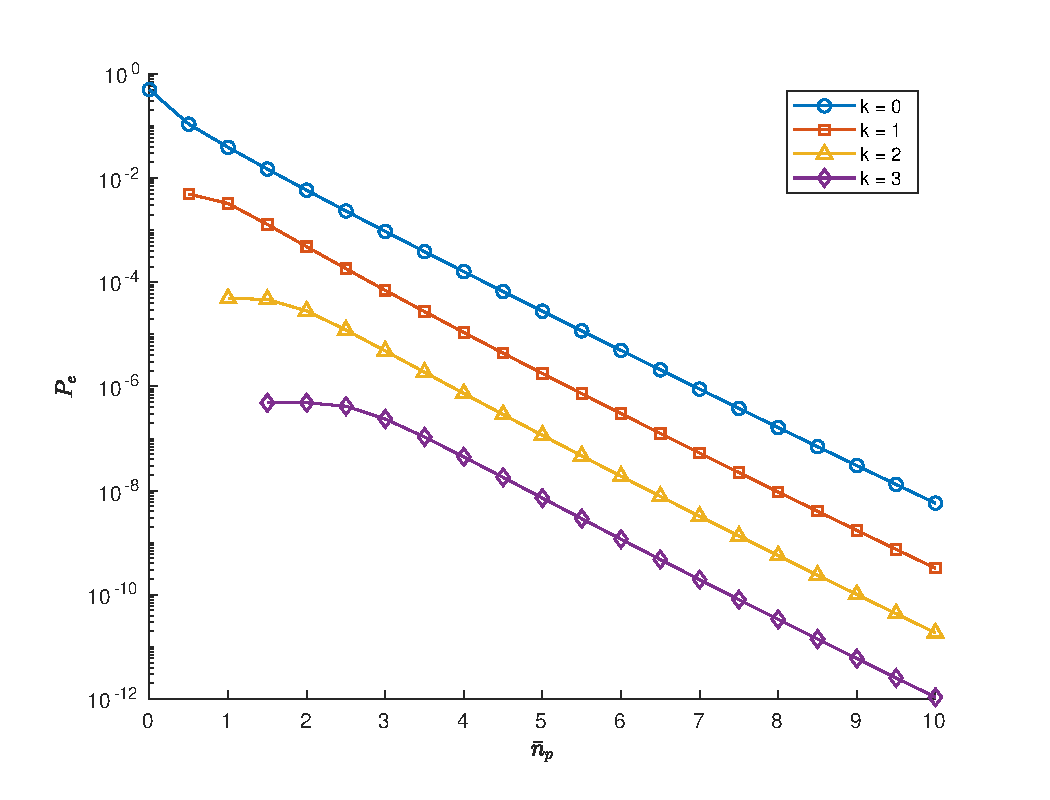
\includegraphics[width=0.8\textwidth]{fig3.1.eps}
            \caption{MDEP for PACS QOOK as function of $\bar{n}_p$ with: $k=0,1,2,3$; $\bar{n}=10^{-2}$; $p_0=p_1=1/2$}
            \label{fig:3.1}
        \end{center}
    \end{figure}
    The MDEP of a quantum OOK system with PACS in function of $\bar{n}_p$ is represented in the figure
    \ref{fig:3.1}. The parameter $\bar{n}_p$ represents the mean number of photons in the system and it is 
    defined as
    \begin{equation*}
        \bar{n}_p=\frac{1}{2} \left(n_{p0}+n_{p1}\right)
    \end{equation*}
    where $n_{pi}$ is the mean number of photons in the state $\Operator{\varXi}_i$.
    The parameter $\bar{n}_p$ is equal to $n_p/2$ for OOK systems and to the average of the $n_p$ for 
    each state for the BPSK system.
    In the y-axes there are the MDEP ($P_e$). The plot was obtained for equiprobable symbols and 
    mean number of thermal photons $\bar{n}=10^{-2}$.  
    The argument of the trace norm $\norm{\cdot}_1$ in the Helstrom bound 
    \ref{eq:HelstromBound}, is an operator in an infinite dimensional Hilbert space; for the 
    simulation, it has been approximated in $N=30$ dimension.
    We can observe that the photon addition improves significantly the performance in terms
    of error probability. Incrasing the value of the parameter $k$ the MDEP of the system 
    transate; the error probability, for the same energy-level, is lower if $k$ is bigger.
    We can notice too that the graphs do not start all from $0$. This is because the minimum
    mean number of photons in a photon added state is not always $0$ as it possible to see in 
    equation \ref{eq:min_np}.  

    \subsection{Quantum BPSK}
    It can be interesting to assess the effect of photon addition in a quantum BPSK system.
    The constellation is given, for a PACS BPSK, by:
    \begin{subequations}\begin{align}
        \Operator{\varXi}_0 &=  \Operator{\varXi}_{\mathrm{th}}^{(k)}(-\mu)\\
        \Operator{\Xi}_1 &=  \Operator{\varXi}_{\mathrm{th}}^{(k)}(\mu).
    \end{align}\end{subequations}
    %
    In absence of noise ($\bar{n}=0$), the MDEP is given by formula \ref{eq:HelstromBPure} where
    \begin{subequations}
        \begin{align}
            \ket{\psi_0}&=\ket*{-\mu^{(k)}},\\
            \ket{\psi_1}&=\ket*{\mu^{(k)}}.
        \end{align}
    \end{subequations}
    %
    The inner product is given, in closed form, by \cite{PACSDisc}:
    \begin{equation}
        \braket*{-\mu^{(k)}}{\mu^{(k)}} = \frac{L_k(\absolutevalue{\mu}^2)}{L_k(-\absolutevalue{\mu}^2)}
        e^{-2\absolutevalue{\mu}^2},
        \label{eq:innerp_nonNoise}
    \end{equation}
    where $L_k(x)$ is the Laguerre polynomial of parameter $k$, evaluate in $x$.
    \begin{figure}[t]
        \begin{subfigure}{0.5\textwidth}
            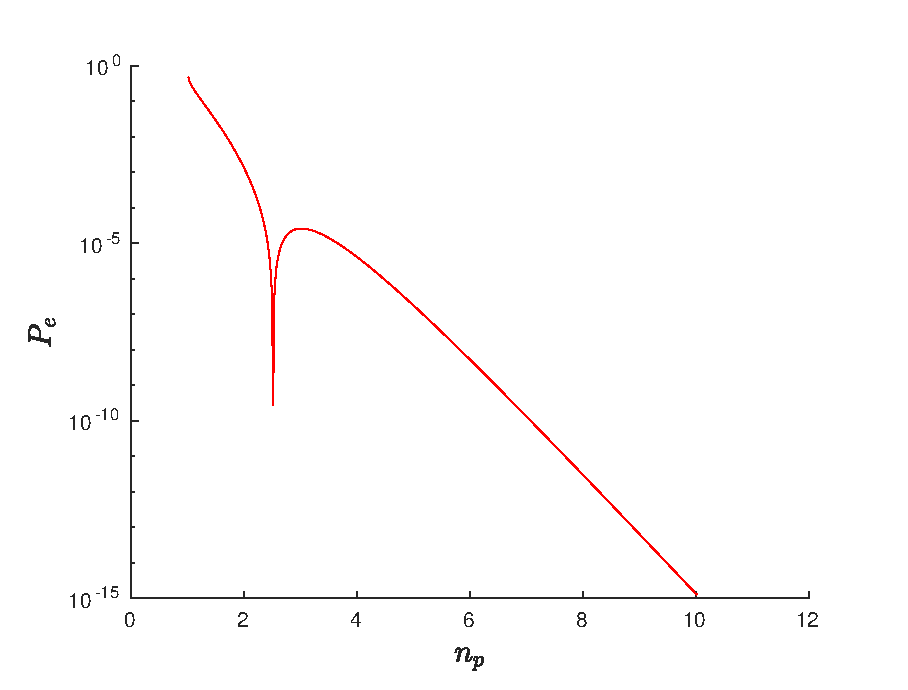
\includegraphics[width=\linewidth]{fig3.2a.eps}
            \caption{$k=1$}
        \end{subfigure}
        %\hspace*{fill}
        \begin{subfigure}{0.5\textwidth}
            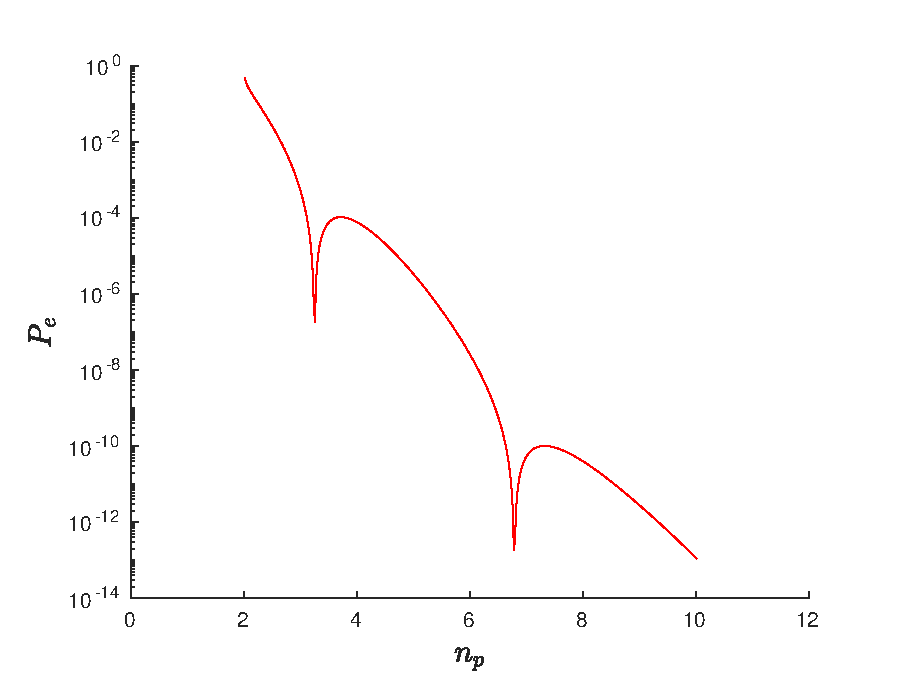
\includegraphics[width=\linewidth]{fig3.2b.eps}
            \caption{$k=2$}
        \end{subfigure}
        \caption{MDEP of quantum BPSK as function of $n_p$, in absence of noise with $N=30$.}
        \label{fig:3.2}
    \end{figure}
    In figure \ref{fig:3.2} the MDEP in absence of noise, for QBPSK with PACS, is plotted for
    $k=1$ and for $k=2$, in function of $n_p$, with $N=30$. It can be noticed that exist $k$ zeros
    in the MDEP plot, where $k$ is the number of photon additions, that corresponds to the zeros
    of $L_k(\absolutevalue{\mu}^2)$ in equation \ref{eq:innerp_nonNoise}.
    The existence of these zeros is not really useful for the design of a quantum communication
    system because their selectivity factors are too high for a phisical implementation. It is, 
    nevertheless, possible to use that in order to evaluate the effect of the thermal noise.
    
    In figure \ref{fig:3.3}, the sluggish performance due to the thermal noise is clear. The plot
    shows the trend of MDEP, for zeros value of $\mu$, in function of $\bar{n}$; the used approximation
    is $N=30$. The MDEP in presence of noise is given using the expression \ref{eq:HelstromBound}.
    We can shown, using the formula \ref{eq:nbar}, that $\bar{n}$ in a real cases in near to zero, the 
    plot show the general trend of the MDEP.
    
    The figure \ref{fig:3.4} show a comparison between a QBPSK system and a QOOK system in terms of 
    MDEP as function of $\bar{n}_p$, i.e. the mean number of photons in the system. 
    The plots are given with $\bar{n}= 10^{-2}$, $N=45$ and equiprobable symbols.
    The obtained result is really intresting: the quantum BPSK system has a sluggish performance due two 
    the photon addition process. At an equal level of energy $\bar{n}_p$, for PACS systems, it is
    possible to find an OOK configuration that maximizes the performance.
    \begin{figure}[t]
        \begin{subfigure}{0.5\textwidth}
            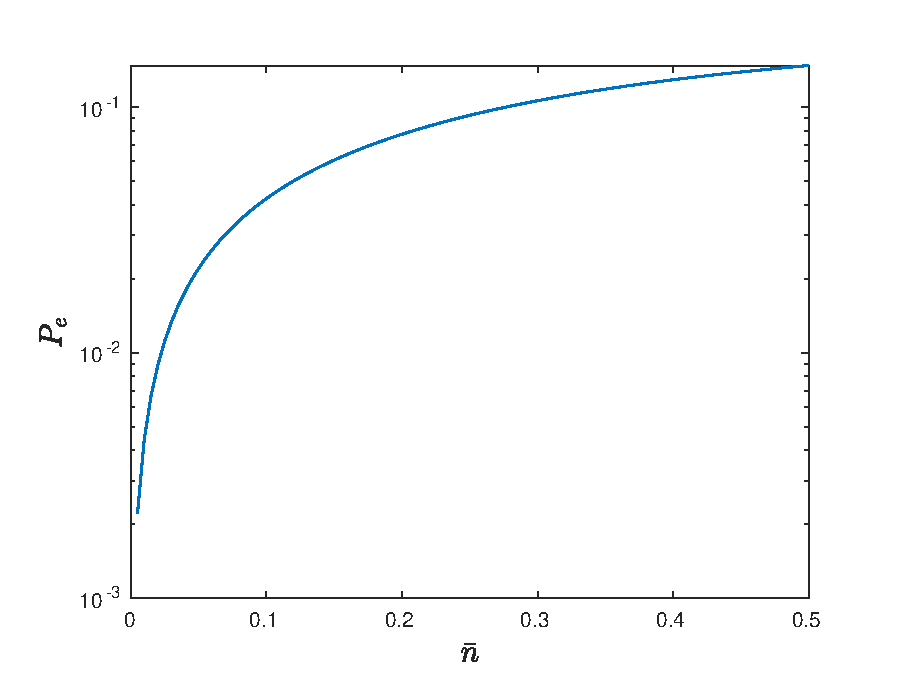
\includegraphics[width=\linewidth]{fig3.3a.eps}
            \caption{$k=1$ and $\mu = 0.54$}
        \end{subfigure}
        %\hspace*{fill}
        \begin{subfigure}{0.5\textwidth}
            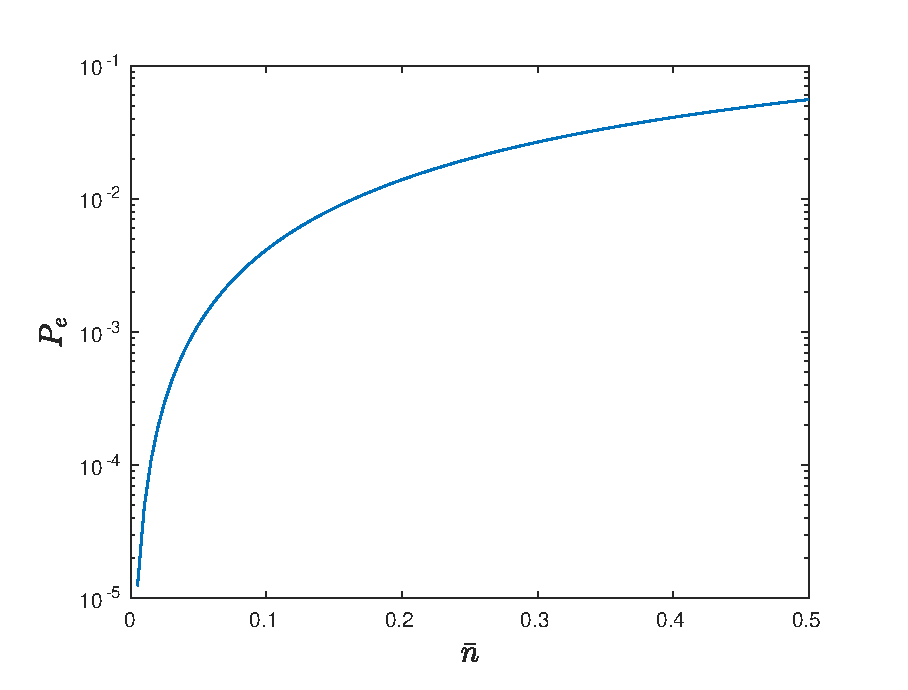
\includegraphics[width=\linewidth]{fig3.3b.eps}
            \caption{$k=2$ and $\mu = 1.58$}
        \end{subfigure}
        \caption{MDEP in corrispondence of MDEP zeros as function of $\bar{n}$ ($N=40$).}
        \label{fig:3.3}
    \end{figure}
    